% IEEE standard conference template; to be used with:
%   spconf.sty  - LaTeX style file, and
%   IEEEbib.bst - IEEE bibliography style file.
% --------------------------------------------------------------------------

\documentclass[letterpaper]{article}
\usepackage{spconf,amsmath,amssymb,graphicx}
\usepackage[utf8]{inputenc}
\usepackage{listings}
\usepackage{color}
\usepackage{enumitem}
\usepackage{url}
\usepackage{hyperref}
\usepackage{units}
\usepackage{float}
\definecolor{dkgreen}{rgb}{0,0.6,0}
\definecolor{gray}{rgb}{0.5,0.5,0.5}
\definecolor{mauve}{rgb}{0.58,0,0.82}

\lstset{frame=tb,
  language=C++,
  aboveskip=3mm,
  belowskip=3mm,
  showstringspaces=false,
  columns=flexible,
  basicstyle={\small\ttfamily},
  numbers=none,
  numberstyle=\tiny\color{gray},
  keywordstyle=\color{blue},
  commentstyle=\color{dkgreen},
  stringstyle=\color{mauve},
  breaklines=true,
  breakatwhitespace=true
  tabsize=3
}

% Example definitions.
% --------------------
% nice symbols for real and complex numbers
\newcommand{\R}[0]{\mathbb{R}}
\newcommand{\C}[0]{\mathbb{C}}

\newcommand{\mypar}[1]{{\\\bf #1.\\}}

% Title.
% ------
\title{Optimization of the Metropolis Algorithm for a Potts Model}
%
% Single address.
% ---------------
\name{Dominik Gresch, Mario Könz} 
\address{Department of Physics\\ ETH Z\"urich\\Z\"urich, Switzerland}

% For example:
% ------------
%\address{School\\
%		 Department\\
%		 Address}
%
% Two addresses (uncomment and modify for two-address case).
% ----------------------------------------------------------
%\twoauthors
%  {A. Author-one, B. Author-two\sthanks{Thanks to XYZ agency for funding.}}
%		 {School A-B\\
%		 Department A-B\\
%		 Address A-B}
%  {C. Author-three, D. Author-four\sthanks{The fourth author performed the work
%		 while at ...}}
%		 {School C-D\\
%		 Department C-D\\
%		 Address C-D}
%

\begin{document}
%\ninept
%
\maketitle
%


\begin{abstract}
\end{abstract}

\section{Introduction}\label{sec:intro}
\subsection{Motivation} 
\subsection{Related work}
\section{Background: Potts Model and the Metropolis Algorithm}\label{sec:background}
\subsection{Potts Model}
The $n$-state Potts model ensemble of spins on a lattice. $n$ different
states are available for each spin. These spins interact only with
their nearest neighbors. The energy of the entire system is given
by:
\[
E=J\sum_{<i,j>}\sigma_{i}^{z}\sigma_{j}^{z}
\]
where $J$ is an interaction constant, $\sigma_{i}^{z}$ the z-component
spin at lattice site i and $<i,j>$ the set of all neighbor-pairs.
If $J<0$ the spins align preferable aligned. The $2$-state Potts
model on a 2D square lattice is identical with the classical Ising
model. For this work the 4-states Potts model on an 3D cubic lattice
with periodic boundary conditions was chosen. The mean properties
of the model can be measured in the following way:
\[
\bar{A}=\sum_{\omega\in\Omega}A(\omega)*p(\omega)
\]
where $\Omega$ denotes the configuration space, $p(\omega)=e^{-\frac{E(\omega)}{k_{b}T}}$
the canonical probability to find a certain configuration $\omega$
in $\Omega$ and $A$ and observable like energy or magnetization.
Due to the large configuration space (increases exponentially with
the number of spins) this sum cannot be calculated directly in a fast
manner. Therefor one needs the metropolis algorithm.
\subsection{Metropolis Algorithm}
The metropolis algorithm is a Markov chain Monte Carlo method \cite{MC} that
allows the calculation of expectation values without having to generate
all configurations $\omega$. After generating a starting state $\omega_{0}$
one does many local spin updates to change the system and generate
the next state $\omega_{1}$. One has make sure that the states are
not correlated, otherwise the error estimations is too small. For
the Potts model, the algorithm consists of following steps:
\begin{enumerate}[noitemsep, topsep = 0pt]
\item Select a random spin $\sigma_{i}^{z}$ from the current configuration
$\omega_{s}$ and change it randomly by $\Delta\sigma_{i}^{z}=\pm1$
to the configuration $\omega_{s}^{*}$
\item Calculate the energy difference $\Delta E_{i}$ and \\ $\frac{p(\omega_{s}^{*})}{p(\omega_{s})}=e^{-\frac{\Delta E_{i}}{k_{b}T}}$
\item Accept the new configuration with the probability
\\ $p_{accept}=min(1,\frac{p(\omega_{s}*)}{p(\omega_{s})})$
\item Repeat step 1 to 3 $m$ times until $\omega_{s}$ and $\omega_{s+m}$
are decorrelated
\item Measure functions of interest on the state $\omega_{s+m}$
\item If the error in the measurements is too large, repeat from step 1\end{enumerate}
\section{Modular Optimizations and Autotuning}\label{sec:yourmethod}
The following section describes the implementation of the Potts model, specifically the splitting into four modules, optimizations performed on those modules and finally autotuning to select the best-performing modules.
\subsection{Modular Structure} Splitting the implementation into four modules (with their respective interfaces) allowed for an efficient workflow. It became possible to optimize parts of the implementation completely independently, which is a great benefit when working in a team. The four modules are as follows:
\begin{itemize}[noitemsep, topsep = 0pt]
\item \textbf{\texttt{SIM}:} Contains the high-level aspects of the metropolis algorithm: Computing probabilities, accepting or rejecting an update, and also calls to the other modules (i.e. requesting random numbers or getting / setting spins).
\item \textbf{\texttt{GRID}:} Takes care of the boundary conditions, i.e. it computes the nearest neighbours of a selected spin.
\item \textbf{\texttt{MATRIX}:} Contains the explicit data format  of the system (e.g. \texttt{std::vector} or \texttt{C array}).
\item \textbf{\texttt{RNG}:} Provides the random numbers. All implementations use a mersenne twister engine.
\end{itemize}
In the following parts, the different optimazation techniques used for each module will briefly be mentioned.
\subsection{\texttt{SIM} optimizations}\label{opt:sim}
\begin{itemize}[noitemsep, topsep = 0pt]
\item \textbf{Probability Precomputation:} Since there is a finite number of possible energy differences $\Delta E$, the probability $p_i = \exp{\left(-\frac{\Delta E_i}{k_B T}\right)}$ of accepting a spin change is precomputed. This may increase memory usage, but gets rid of any floating point computation.
\item \textbf{Interleaving:} The calls to the random number generator (picking the spin location) and the actual computation is interleaved amongst two steps. This allows prefetching, i.e. the data for the next step can be loaded during the current step.
\item \textbf{Explicit Prefetching:} Instead of leaving it up to the Compiler and/or Hardware, the prefetching is done explicitly. 
\end{itemize}
\subsection{\texttt{GRID} optimizations} A \textbf{lookup table} (one array for each space direction) was used to get the nearest neighbour indices efficiently. This method is useful mainly because it replaces the potentially expensive check for the boundary condition.
\subsection{\texttt{MATRIX} optimizations} The main concern with the \texttt{MATRIX} module storing the system in a memory - efficient way. Also, since the access to spins is random, the \texttt{MATRIX} is the only way we can hope to achieve locality (between one position and its nearest neighbours). The following optimizations have been done:
\begin{itemize}[noitemsep, topsep = 0pt]
\item\textbf{Compression:} Since each spin can only be in one of four states, it can be described using only 2 \texttt{bits}. This can be used to shrink the system's size in memory by a factor of $4$ (compared to using one \texttt{byte} per spin).
\item{\textbf{Z - order:}} Bit interleaving in the three indices is used to increase locality amongst a spin and its nearest neighbours.
\end{itemize}
\subsection{\texttt{RNG} optimizations} \label{opt:rng}
\begin{itemize}[noitemsep, topsep = 0pt]
\item \textbf{Economic use:} Since many of the random numbers used only are a few \texttt{bits} long, the \texttt{std::mt19937} implementation (which uses $32 \mathtt{bit}$ for each random number at least) can be optimized greatly by using all the bits in each generated random number (with some overhead for splitting up the random numbers).
\item \textbf{MKL:} The underlying Mersenne twister engine was exchanged for the MKL implementation \cite{MKL} (whilst still using the method of economic use described before).
\end{itemize}
\subsection{Autotuning}
Many of the optimizations seen in sections \ref{opt:sim} - \ref{opt:rng} perform well only under certain conditions (i.e. at certain system sizes and temperatures). For example, using Z - order might be great at large sizes, but the overhead for computing the index is too large for smaller ones. \\
The modular structure of the code provides the ideal grounds for tackling this problem using an autotuning approach:\\
For a fixed number of sizes, the optimized combination of modules is searched (either by doing a full sweep over all the combinations, or - much faster - by iteratively exchanging one module whilst keeping the others fixed). This installation routine creates a header file (\texttt{install.hpp}) containing template specialisations, as seen in Listing \ref{listing1}.
\begin{lstlisting}[caption = {example for a template specialisation}, label = listing1]
template<>
struct opt<150> {
    template<int S>
    using impl = greschd_v3_sim::impl<S, S, S, addon::mkl_mt_rng, msk_v1_pbc, msk_v2_dynamic_zip>; 
};
\end{lstlisting}
For an arbitrary size $N$, the implementation will then choose the appropriate specialisation (that is, the one with size closest to $N$) by use of type traits, as indicated in Listing \ref{sizehelper}.
\begin{lstlisting}[label = sizehelper, caption = {size\_helper, part of the type traits}]
template<int S, int N, bool B>
struct size_helper {
    static constexpr int size = size_helper<S, N - 1, S >= (sizes[N] + sizes[N - 1])/ 2 >::size;
};
\end{lstlisting}
\section{Experimental Results}\label{sec:exp}
This section describes the different measurements that were performed and their results. After introducing the platforms that were used and some notation, the impact each optimisation has on runtime is studied. Finally, the results of screening all module combinations and the performance of the auto - tuned code is shown.
\subsection{Experimental setup} \label{exp:setup}
The two platforms used are shown in Table \ref{platforms}. 
\begin{table}[h]
\begin{tabular}{lll}
 & \textbf{Haswell} & \textbf{Wolfdale}\\\hline
\textbf{Architecture} & Intel Core i7 & Intel Core 2\\\hline
\textbf{Frequency} & $\unit[2.4]{GHz}$ & $\unit[2.4]{GHz}$\\\hline
\textbf{OS} & Ubuntu 13.10 & Ubuntu 14.04\\\hline
\textbf{Compiler} & gcc 4.8.1 & gcc 4.8.1\\\hline
 & -std=c++11  & -std=c++11  \\
\textbf{Flags}& -DNDEBUG & -DNDEBUG \\
& -O3  &  -O3 \\
& -march=core-avx2 & -march=core2 \\
\end{tabular}
\caption{Platforms used for the measurements}
\label{platforms}
\end{table}
\newline For all measurements, the rdtsc command was used to determine the runtime. In the roofline measurements, the memory traffic was measured with perfplot \cite{PERFPLOT}. Additionally, VTune, perf and gprof were used for profiling during development.
also used.\newline
Measurements showing the splitting of runtime amongst the different modules is achieved by starting / stopping the time measurement between different tasks in the algorithm. This may to some extent influence the total runtime by inhibiting out-of-order computation.\newline
Runtime of \texttt{GRID} and \texttt{MATRIX} is measured together, but split into accessing selected spin itself (single spin, s.s.) and accessing its nearest neighbours (n.n.). \newline
The exact configuration of modules used in a measurement is noted using a four - digit index corresponding to (SIM, GRID, MATRIX, RNG) as listed in Table \ref{modlist} (with optimisations as described in Sec. \ref{sec:yourmethod}):
\begin{table}[h]
\begin{tabular}{ll|l}
& \textbf{index} & \textbf{optimisations} \\\cline{2-3}
\textbf{SIM:} \\\hline
& \textbf{0} & baseline \\\cline{2-3}
& \textbf{1} & probability precomputation\\\cline{2-3}
& \textbf{2} & 1 \& interleaving \\\cline{2-3}
& \textbf{3} & 2 \& explicit prefetching\\\cline{2-3}
\textbf{GRID:}\\\hline
& \textbf{0} & baseline \\\cline{2-3}
& \textbf{1} & boundary lookup table \\\cline{2-3}
\textbf{MATRIX:}\\\hline
& \textbf{0} & baseline (\texttt{std::vector}) \\\cline{2-3}
& \textbf{1} & C array \\\cline{2-3}
& \textbf{2} & compressed \\\cline{2-3}
& \textbf{3} & Z - order \\\cline{2-3}
& \textbf{4} & compressed \& Z - order\\\cline{2-3}
\textbf{RNG:} \\\hline
& \textbf{0} & baseline (STL mt)\\\cline{2-3}
& \textbf{1} & economic use \\\cline{2-3}
& \textbf{2} & 1 \& MKL engine\\\cline{2-3}
\end{tabular}
\caption{List of Modules}
\label{modlist}
\end{table}
\subsection{Results: SIM optimization}
Figures \ref{SIM:Wolf:20} and \ref{SIM:Has:20} show the runtime partition of the single spin update. All modules except SIM are the same. The baseline-module computes the Boltzmann factors each time, while the second module precomputes these probabillities. The amount of cycles needed for the SIM part is reduced on both systems. On Haswell, this shows a $2$x speedup for a system with side length $N = 20$.
	\begin{figure}[H]\centering
	  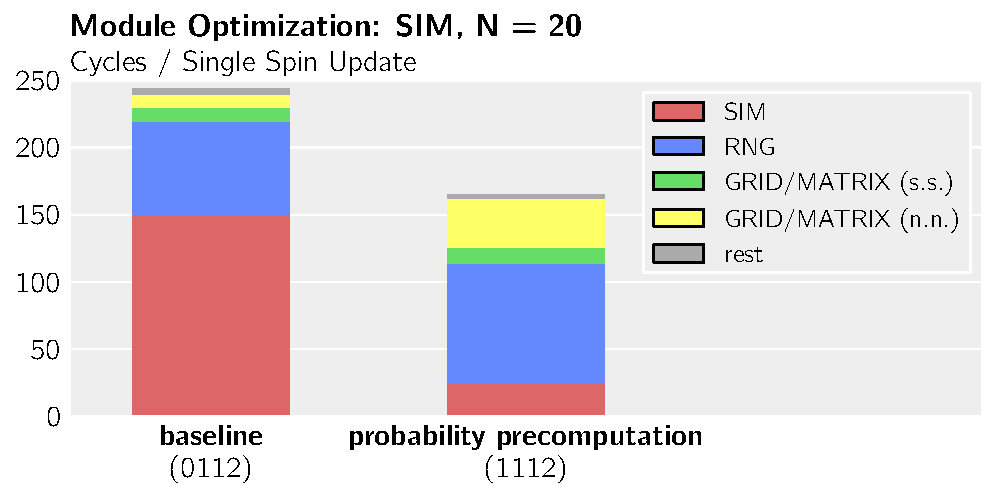
\includegraphics[width = 8.36cm]{plots/msk_20_2.pdf}
	  \caption{Speedup by probability precomputation, on Wolfdale}
	  \label{SIM:Wolf:20}
	\end{figure}
	\begin{figure}[h]\centering
	  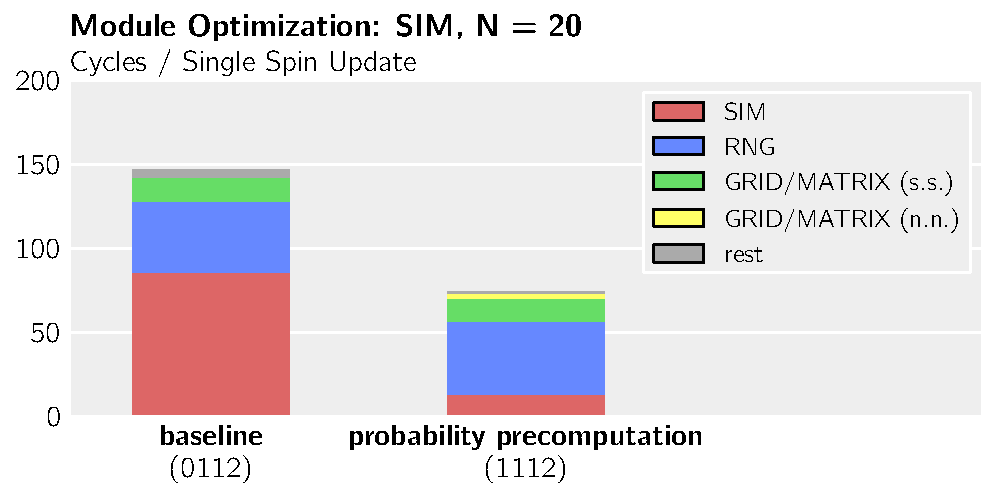
\includegraphics[width = 8.36cm]{plots/dg_20_2.pdf}
	  \caption{Speedup by probability precomputation, on Haswell}
	  \label{SIM:Has:20}
	\end{figure}
\subsection{Results: GRID optimization}
Storing the boundary condition in a lookup table doesn't show a very significant speedup in terms of total runtime. However, nearest neighbour access - the part that is influenced most by the improvement - is sped up by roughly $2$x for sidelength $N = 20$ (see Fig. \ref{GRID:Wolf:20} and \ref{GRID:Has:20}).
	\begin{figure}[h]\centering
	  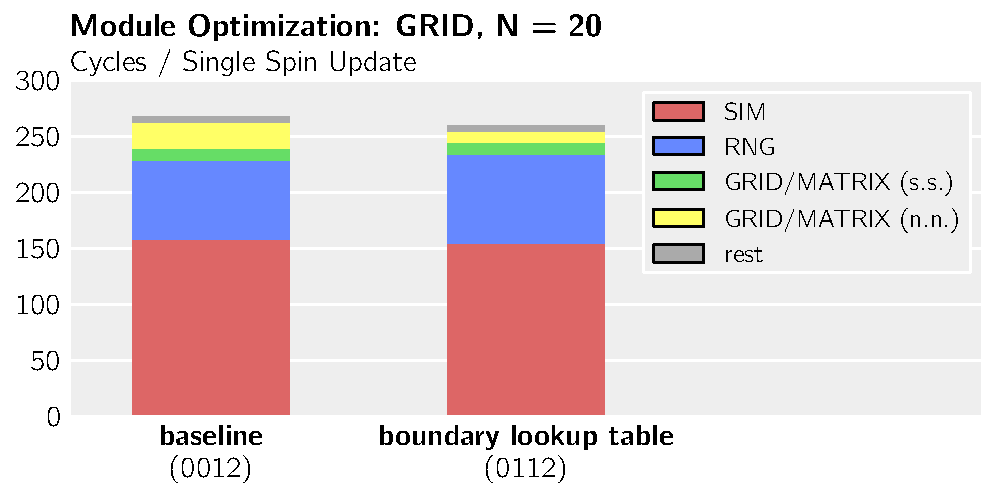
\includegraphics[width = 8.36cm]{plots/msk_20_1.pdf}
	  \caption{Influence on runtime by using a boundary lookup table (\texttt{GRID} optimisation), on Wolfdale}
	  \label{GRID:Wolf:20}
	\end{figure}
	\begin{figure}[h]\centering
	  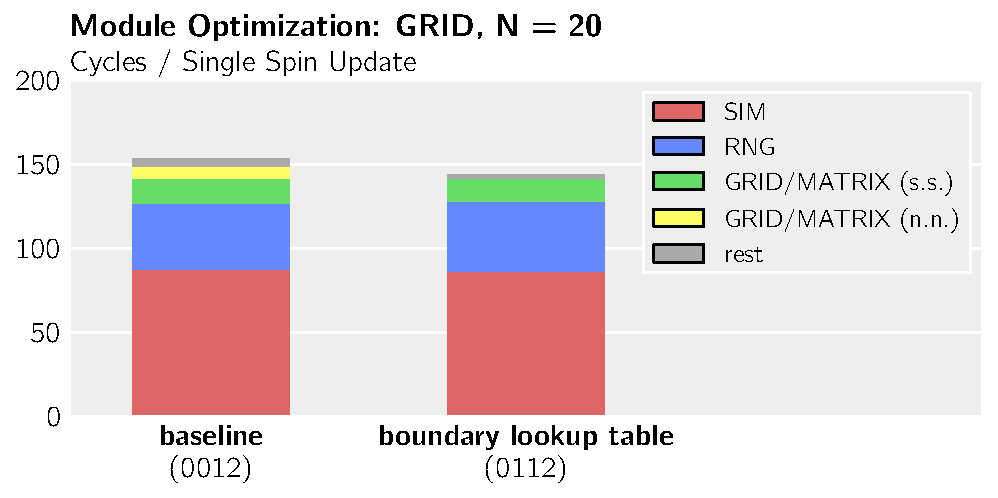
\includegraphics[width = 8.36cm]{plots/dg_20_1.pdf}
	  \caption{Influence on runtime by using a boundary lookup table (\texttt{GRID} optimisation), on Haswell}
	  \label{GRID:Has:20}
	\end{figure}
\subsection{Results: MATRIX optimization}
The impact compression and Z-order have on the runtime is clearly size - dependent: For a small system ($N = 20$, $8000$ spins, on Wolfdale), the influence of compression is negligible and the overhead for using Z - order is larger than the gain (see Fig. \ref{MATRIX:Wolf:20}).
	\begin{figure}[h]\centering
	  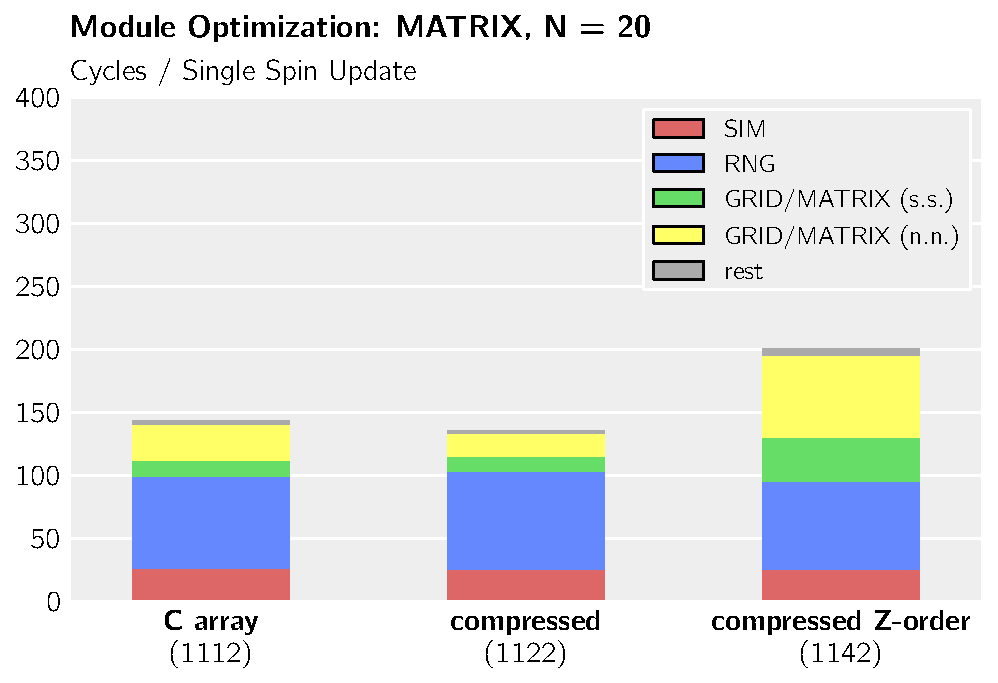
\includegraphics[width = 8.36cm]{plots/msk_20_3.pdf}
	  \caption{Different \texttt{MATRIX} optimisations for $N = 20$, on Wolfdale}
	  \label{MATRIX:Wolf:20}
	\end{figure}\newline
At larger sizes, as the impact of accessing the spins increases, compresssion and Z-order both become significant improvements (see Fig. \ref{MATRIX:Wolf:300}). This improvement is most noticeable when the system starts running out of last level cache. At those sizes, the compressed version might still fit into LLC and hence perform much better.
	\begin{figure}[h]\centering
	  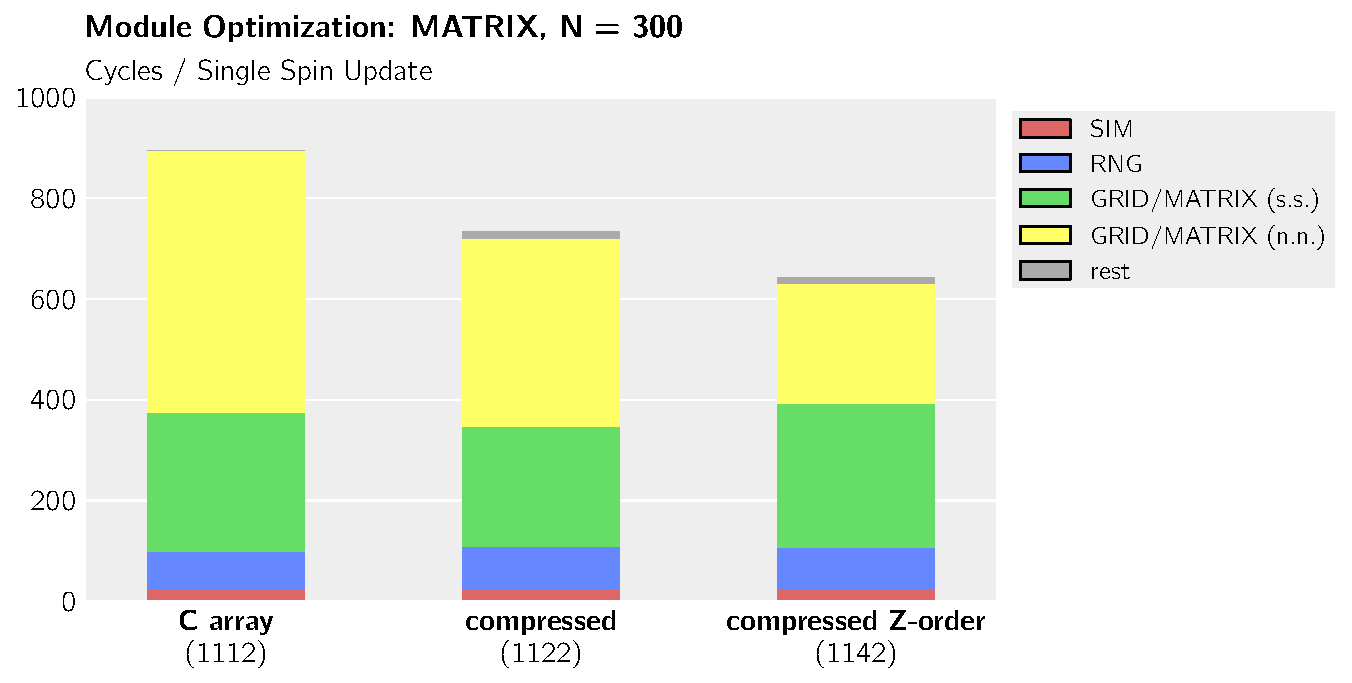
\includegraphics[width = 8.36cm]{plots/msk_300_3.pdf}
	  \caption{Different \texttt{MATRIX} optimisations for $N = 300$, on Wolfdale}
	  \label{MATRIX:Wolf:300}
	\end{figure}\newline
On Haswell, it can be observed that even for large sizes ($N=1000$, $10^9$ spins), accessing the nearest neighbours takes next to no time (see Fig. \ref{MATRIX:Has:1000}). This might be due to the prefetching in Haswell, which could load the neighbours into Cache as soon as the position of the single spin is known. However, this would still cost memory bandwidth, but go undetected by this measuring scheme since it happens out-of-order (see Sec. \ref{exp:setup}). 
	\begin{figure}[h]\centering
	  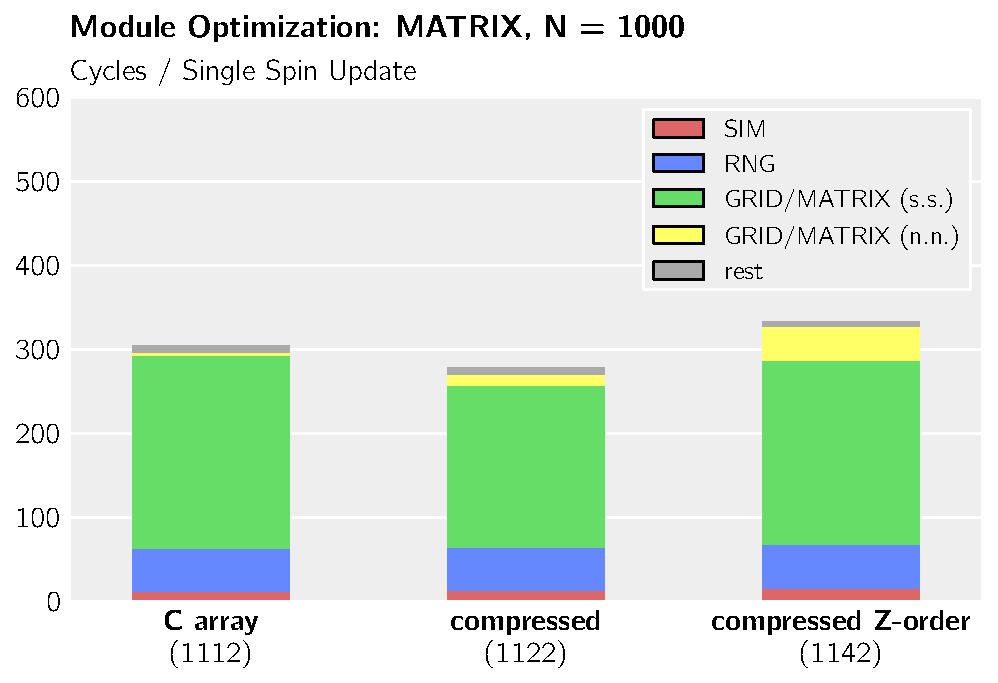
\includegraphics[width = 8.36cm]{plots/dg_1000_3.pdf}
	  \caption{Different \texttt{MATRIX} optimisations for $N = 1000$, on Haswell}
	  \label{MATRIX:Has:1000}
	\end{figure}
\subsection{Results: RNG optimization}
Economic use of the random numbers shows significant impact ($>2$x for small sizes). Using the MKL engine however shows some speedup, but not a negligible one (see Fig. \ref{RNG:Has:20}).
	\begin{figure}[h]\centering
	  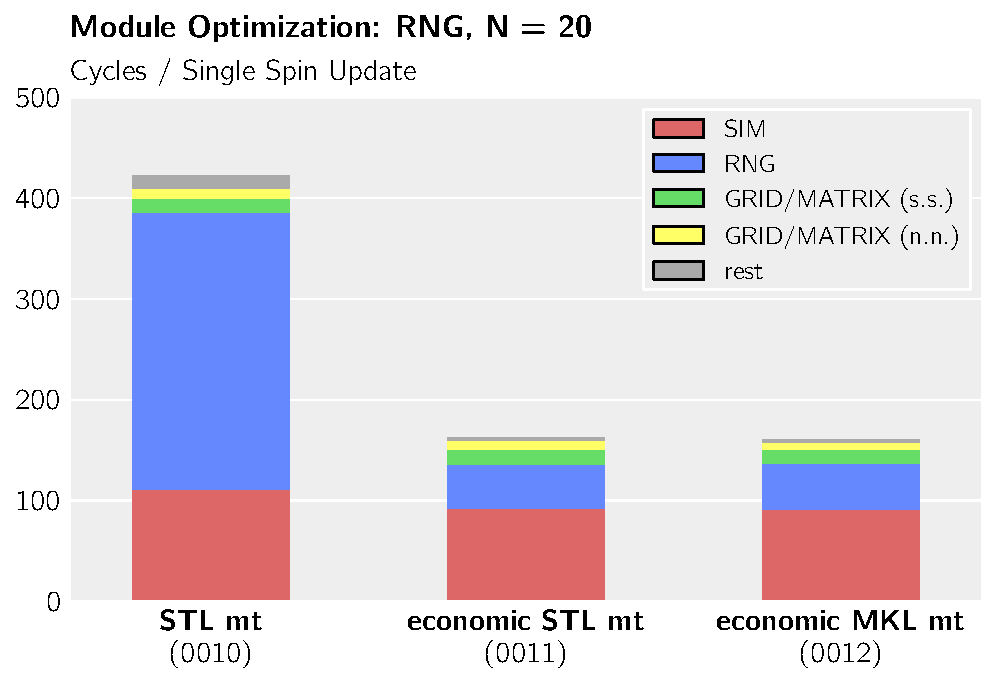
\includegraphics[width = 8.36cm]{plots/dg_20_0.pdf}
	  \caption{Runtime using different \texttt{RNG} modules, on Haswell}
	  \label{RNG:Has:20}
	\end{figure}
\subsection{Results: Autotuning}
	\begin{figure}[h]\centering
	  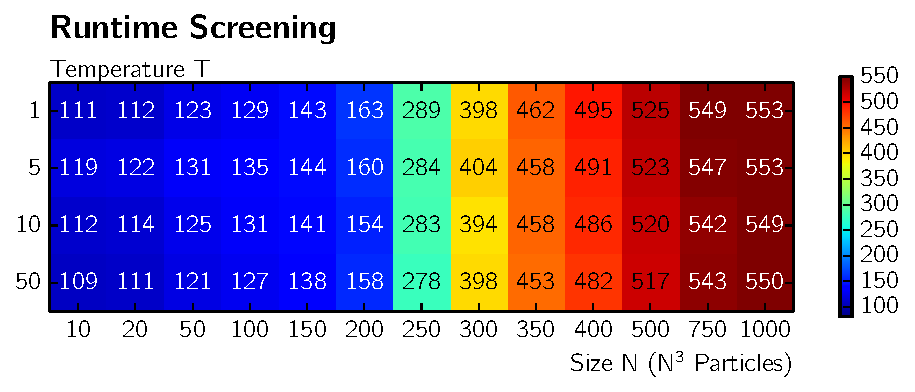
\includegraphics[width = 8.36cm]{plots/matrix_msk.pdf}
	  \caption{Performance Screen, Wolfdale}
	\end{figure}
	\begin{figure}[h]\centering
	  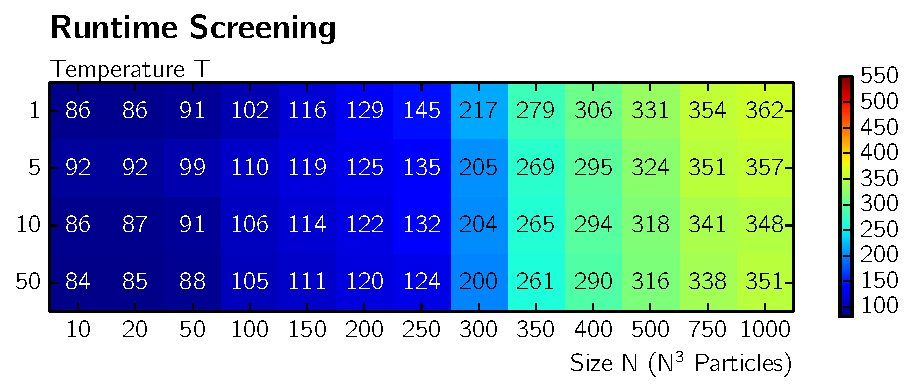
\includegraphics[width = 8.36cm]{plots/matrix_dg.pdf}
	  \caption{Performance Screen, Haswell}
	\end{figure}
	\begin{figure}[h]\centering
	  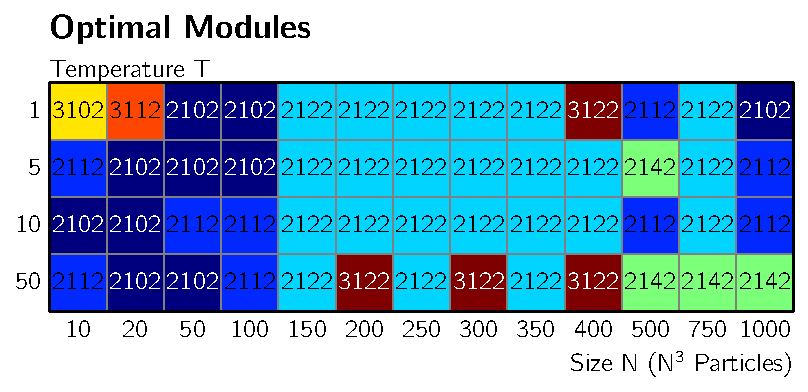
\includegraphics[width = 8.36cm]{plots/module_msk2.pdf}
	  \caption{Modules, Wolfdale}
	\end{figure}
	
	\begin{figure}[h]\centering
		  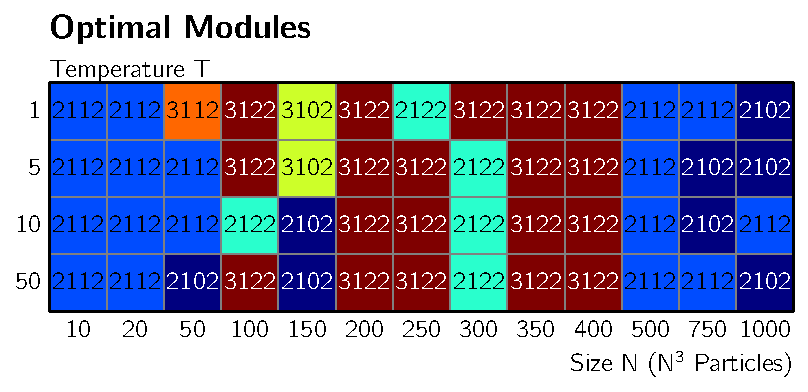
\includegraphics[width = 8.36cm]{plots/module_dg2.pdf}
		  \caption{Modules, Haswell}
	\end{figure}
	

\subsection{Results: Performance}
	\begin{figure}[h]\centering
		  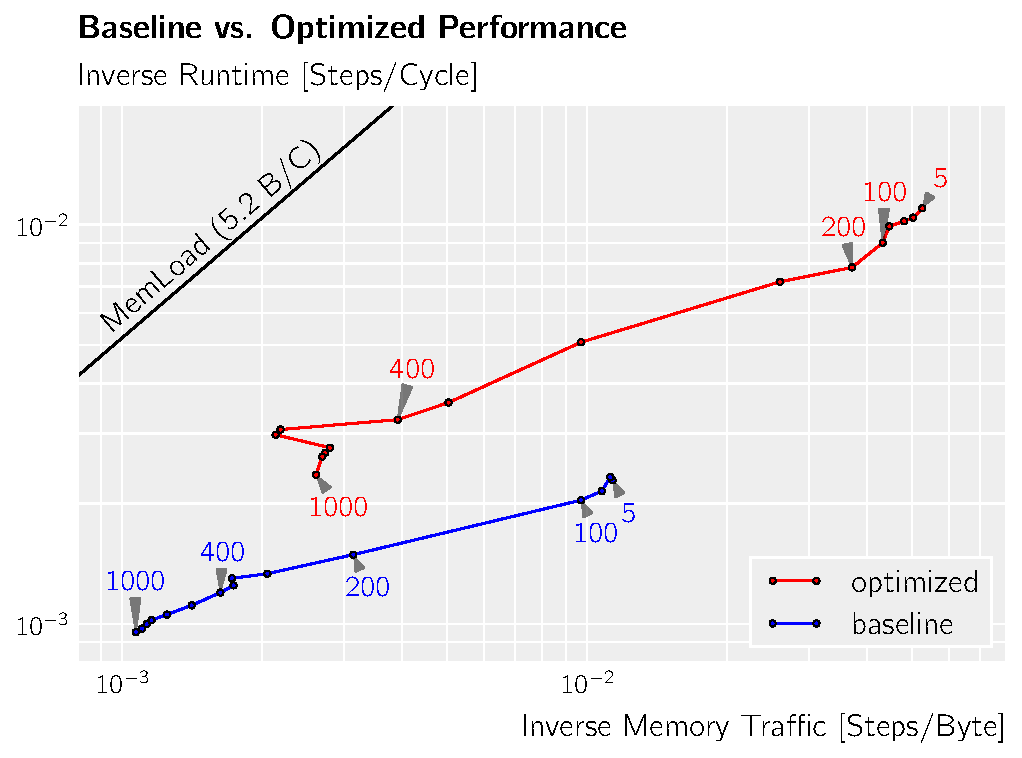
\includegraphics[width = 8.36cm]{plots/roofline_0.pdf}
		  \caption{Roofline, opt. vs baseline, Haswell}
	\end{figure}
	\begin{figure}[h]\centering
		  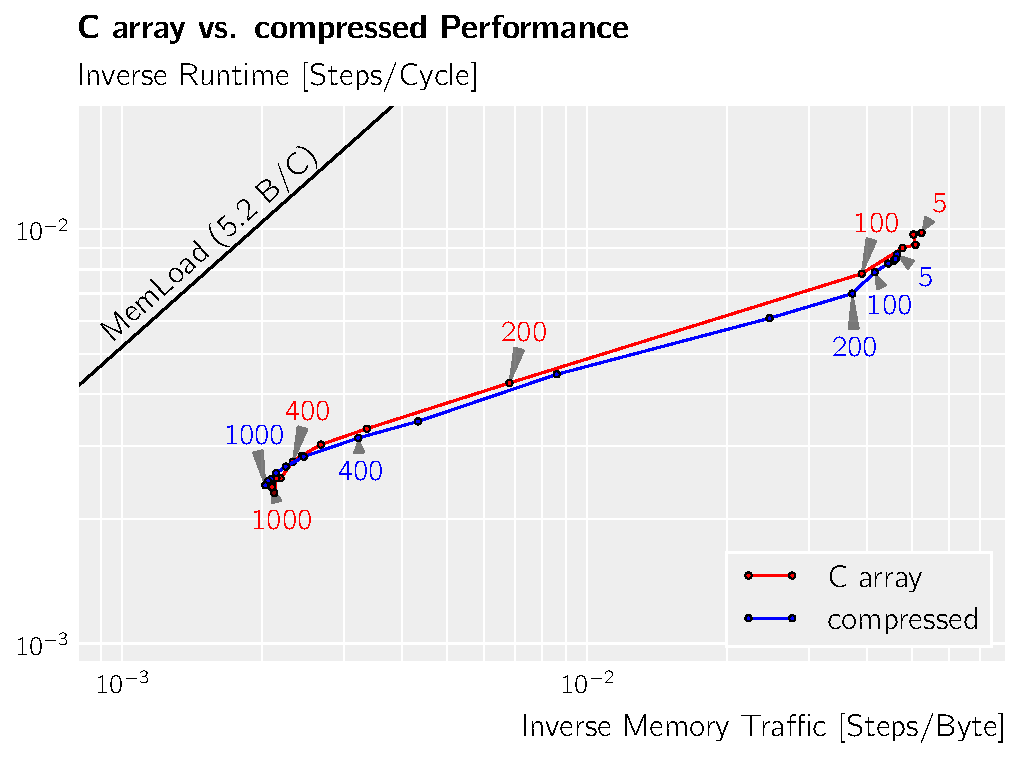
\includegraphics[width = 8.36cm]{plots/roofline_1.pdf}
		  \caption{Roofline, C array and compressed, Haswell}
	\end{figure}

\section{Conclusions}

\bibliographystyle{IEEEbib}
\bibliography{bibl_conf}

\end{document}

